\documentclass[dvipsnames,tikz]{standalone}
\usepackage{amsmath}
\usepackage{arevmath}
\usepackage{xcolor}
\usepackage{tikz}
\usetikzlibrary{calc}
\usetikzlibrary{decorations.pathreplacing,calligraphy,3d}

\tikzset{main/.style={draw=black, circle, color=black}}


\begin{document}
	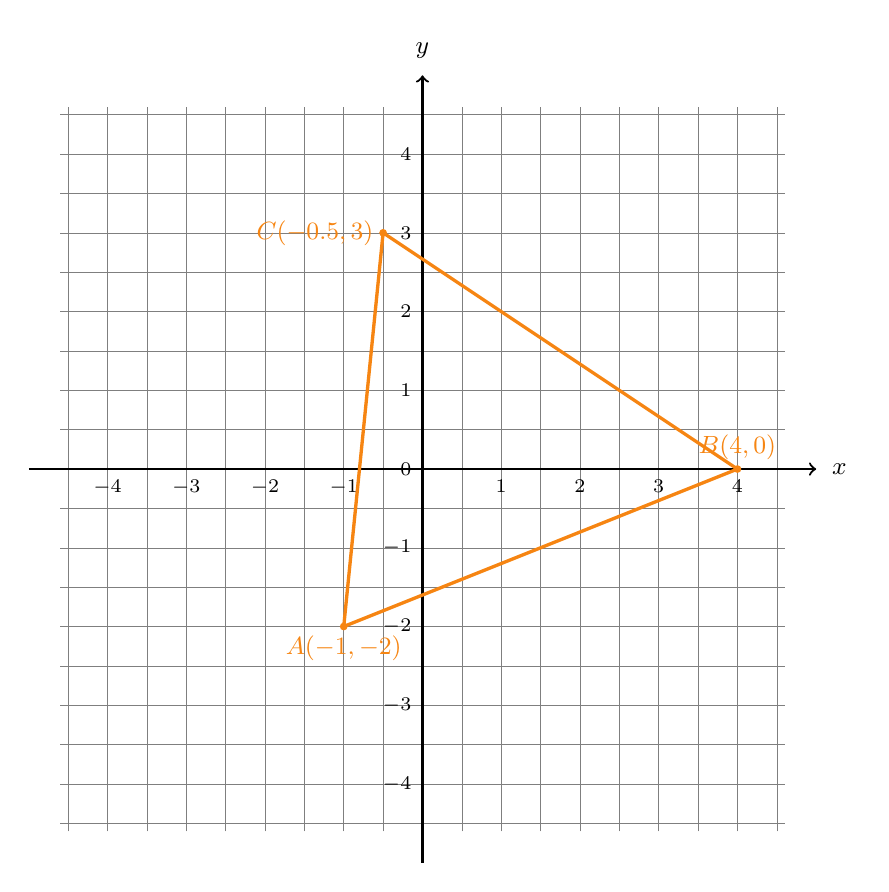
\begin{tikzpicture}[font=\small, tl/.style = {black, inner sep=1pt, font=\scriptsize} ]
	% grid
	\draw[main, very thin, xstep=0.5, ystep=0.5, semitransparent] (-4.6,-4.6) grid (4.6,4.6);
	
	% y tick label
	\foreach \y in {-4,...,4} {\node[ tl, black, left=1mm] at (0,\y) {$\y$};}
	% x tick label
	\foreach \x in {-4,...,-1, 1,2, 3, 4} {\node[tl, black, below=1mm] at (\x,0) {$\x$};}

	% axes
	\draw[main, ->,thick] (-5,0) -- (5,0) node[right] {$x$};
	\draw[main, ->,thick] (0,-5) -- (0, 5) node[above] {$y$};
	
	\draw[very thick, BurntOrange] (-1,-2) -- (4,0) -- (-0.5,3) -- cycle;
	\fill[BurntOrange] (-1,-2) circle (1.4pt) node [below] {$A(-1,-2)$};
	\fill[BurntOrange] (4,0) circle (1.4pt) node [above] {$B(4,0)$};
	\fill[BurntOrange] (-0.5,3) circle (1.4pt) node [left] {$C(-0.5,3)$};
\end{tikzpicture}
\end{document}